\documentclass[doublecol]{epl2}
% or \documentclass[page-classic]{epl2} for one column style
\graphicspath{{figures/}}

\title{A novel scaling indicator of early warning signals 
helps anticipate tropical cyclones}
\shorttitle{A novel scaling indicator of early warning signals} %Insert here a short version of the title if it exceeds 70 characters

\author{J. Prettyman\inst{1,2} \and T. Kuna\inst{1} \and V. Livina\inst{2}}
\shortauthor{J. Prettyman \etal}

\institute{                    
  \inst{1} University of Reading, Whiteknights, Reading, RG6 6AX, UK\\
  \inst{2} National Physical Laboratory, Hampton road, 
Teddington, TW11 0LW, UK
}
\pacs{05.45.Tp}{Time series analysis in nonlinear dynamics}
\pacs{05.45.-a}{Bifurcation: nonlinear dynamics}
\pacs{02.30.Oz}{Bifurcation theory}


\abstract{
Tipping events in dynamical systems have been studied in many 
contexts, often modelled by the decay of critical modes, 
system states which are tending towards bifurcation, characterised 
by increased return times to stable equilibria. Temporal scaling 
properties of time series data can be used to detect the presence 
of a critical mode by estimating the decay rate, and indicators of 
changes in these properties may therefore be used to provide an early 
warning signal (EWS) for an impending tipping event. The lag-1 
autocorrelation function (ACF(1)) indicator and the detrended 
fluctuation analysis (DFA) indicator have previously been used 
in such a way; in this paper we introduce a novel scaling indicator 
based on the decay rate of the power spectrum (PS). 
We compare the ACF(1), DFA- and PS-indicators using artificial data; 
data from a model which includes a bifurcation point; and sea-level 
pressure data along the paths of 14 tropical cyclones. 
By using the PS-indicator with such data, we show that the new 
indicator may be used to provide an EWS in a context where the 
ACF(1)- and DFA-indicators fail.}

\usepackage{color}
\def\bb{\begin{color}{blue}}
\def\br{\begin{color}{red}}
\def\eb{\end{color}\ }

\begin{document}
\bibliographystyle{eplbib}

\maketitle

\section{Introduction}\label{sec_intro}

Tipping events have been studied in many climatological and 
ecological contexts 
\cite{scheffer2001, livina2011, dakos2012, ashwin2012, gsell2016, 
ditlevsen17}. 
These tipping points, which may be thought of as qualitative 
changes in the underlying dynamical systems, have been modelled 
by the decay of stable equilibria \cite{scheffer2009}, which we 
refer to as critical modes as they approach the critical threshold 
leading to a bifurcation. They are identified by their rate of decay, 
known as critical slowing down, which can be estimated from the 
scaling properties of the system time series in the proximity of the 
tipping point.

The authors of \cite{scheffer2009} associate critical slowing down 
with increasing return times to the critical mode, which is modelled 
as an autoregressive process and thus the lag-1 autocorrelation 
function (ACF) is used to detect the critical slowing down. 
The lag-1 ACF, or ACF(1), can therefore be used as a predictive 
indicator of tipping points \cite{held2004}, or early warning signal.

Furthermore, due to the scaling properties, it is possible to use 
longer-term autocorrelations of a time series as an indicator, 
the power-law decay rate of the ACF with increasing time lag is 
one such example. Detrended fluctuation analysis (DFA) averages 
the variance over non-overlapping segments of length $s$ of a 
time series after subtracting an order $n$ polynomial 
trend~\cite{kantelhardt2001}.
%[Kantelhardt et al., 2001]. 

Since during the critical slowing down of the system
dynamics DFA provides a method to study the scaling properties, 
similarly to the ACF, the DFA scaling indicator has been introduced 
as an alternative to the ACF(1)-indicator \cite{livina2007}. 
Both the ACF(1) and DFA-indicators have been shown to detect 
early warning signals of bifurcations and tipping points in a 
variety of systems \cite{dakos2008, lenton2012}.

In this paper we propose a novel scaling indicator based on the 
power-law decay rate of the power spectrum (PS), as the PS scaling 
exponent is related to the ACF and DFA scaling exponents 
\cite{kantelhardt2001}. We introduce the PS-indicator then compare 
the performance of the PS-indicator to the ACF(1)- and 
DFA-indicators using an artificially constructed time series. 
This allows us to compare the responses to changing 
scaling exponent $\beta$. We further compare the ACF(1)-, 
DFA- and PS-indicators when applied to a time series from a classic 
example of a model with a pitchfork bifurcation, where we would at 
least expect that the ACF(1)-indicator would provide a very clear EWS. 
We then apply the three scaling indicators to sea-level pressure 
data along the paths of 14 tropical cyclones, in order to assess 
the suitability of these methods, particularly the PS-indicator, 
in providing an EWS in such a geophysical context. 
In performing these experiments using artificial and 
real geophysical data, we aim to show that the new PS-indicator 
performs similarly to the other well-studied indicators, as we 
expect based on the analytical relationship \cite{kantelhardt2001}. 
Finally, we comment on the sensitivity of the PS-indicator method 
to the window-size parameter.

\section{Scaling properties of time series}
\label{subsec_scalingproperties}

Scaling properties of time series can be measured using three techniques: 
the autocorrelation function (ACF), detrended fluctuation analysis~(DFA) 
and the power spectrum \cite{bak1988, kantelhardt2001}. 
These three methods are illustrated in fig.~\ref{fig1} where we plot 
a time series of artificial data and three scaling curves. 
The data is a length 10000 red-noise series, with power spectrum 
scaling exponent of $\beta =0.85$. To generate this series, 
we first sample from a Gaussian distribution to approximate 
white noise, $X(t)$, we then take the fast Fourier transform 
of this white noise series (denoted $\hat{X}(f)$) and then 
transform this by  
\begin{equation} 
\hat{Y}(f) := \hat{X}(f)\sqrt{f^{-\beta}}.\label{eqn_inverse_fourier} 
\end{equation} 
Finally, we use the inverse fast Fourier transform to obtain the 
time series $Y(t)$, which has power spectrum $S(f)$ proportional 
to $f^{-\beta}$.

The ACF scaling exponent ($\gamma$), fig. \ref{fig1}b, is the 
power-law decay rate of the autocorrelation function with 
increasing lag ($s$) \cite{kantelhardt2001}. Denote by $C(s)$ 
the autocorrelation with lag $s$ of time series $X$, then the 
scaling is defined as 
\begin{equation} 
C(s) \sim s^{-\gamma}, \label{ACF_scaling_equation} 
\end{equation} 
for long-range correlations. Following~\cite{livina2007}, 
we measure the exponent in the range $10\leq s \leq 100$. 
For short-range correlated data, $C(s)$ decays 
exponentially and only ACF(1) is indicative of data variability 
in proximity to a tipping point.

\begin{figure}
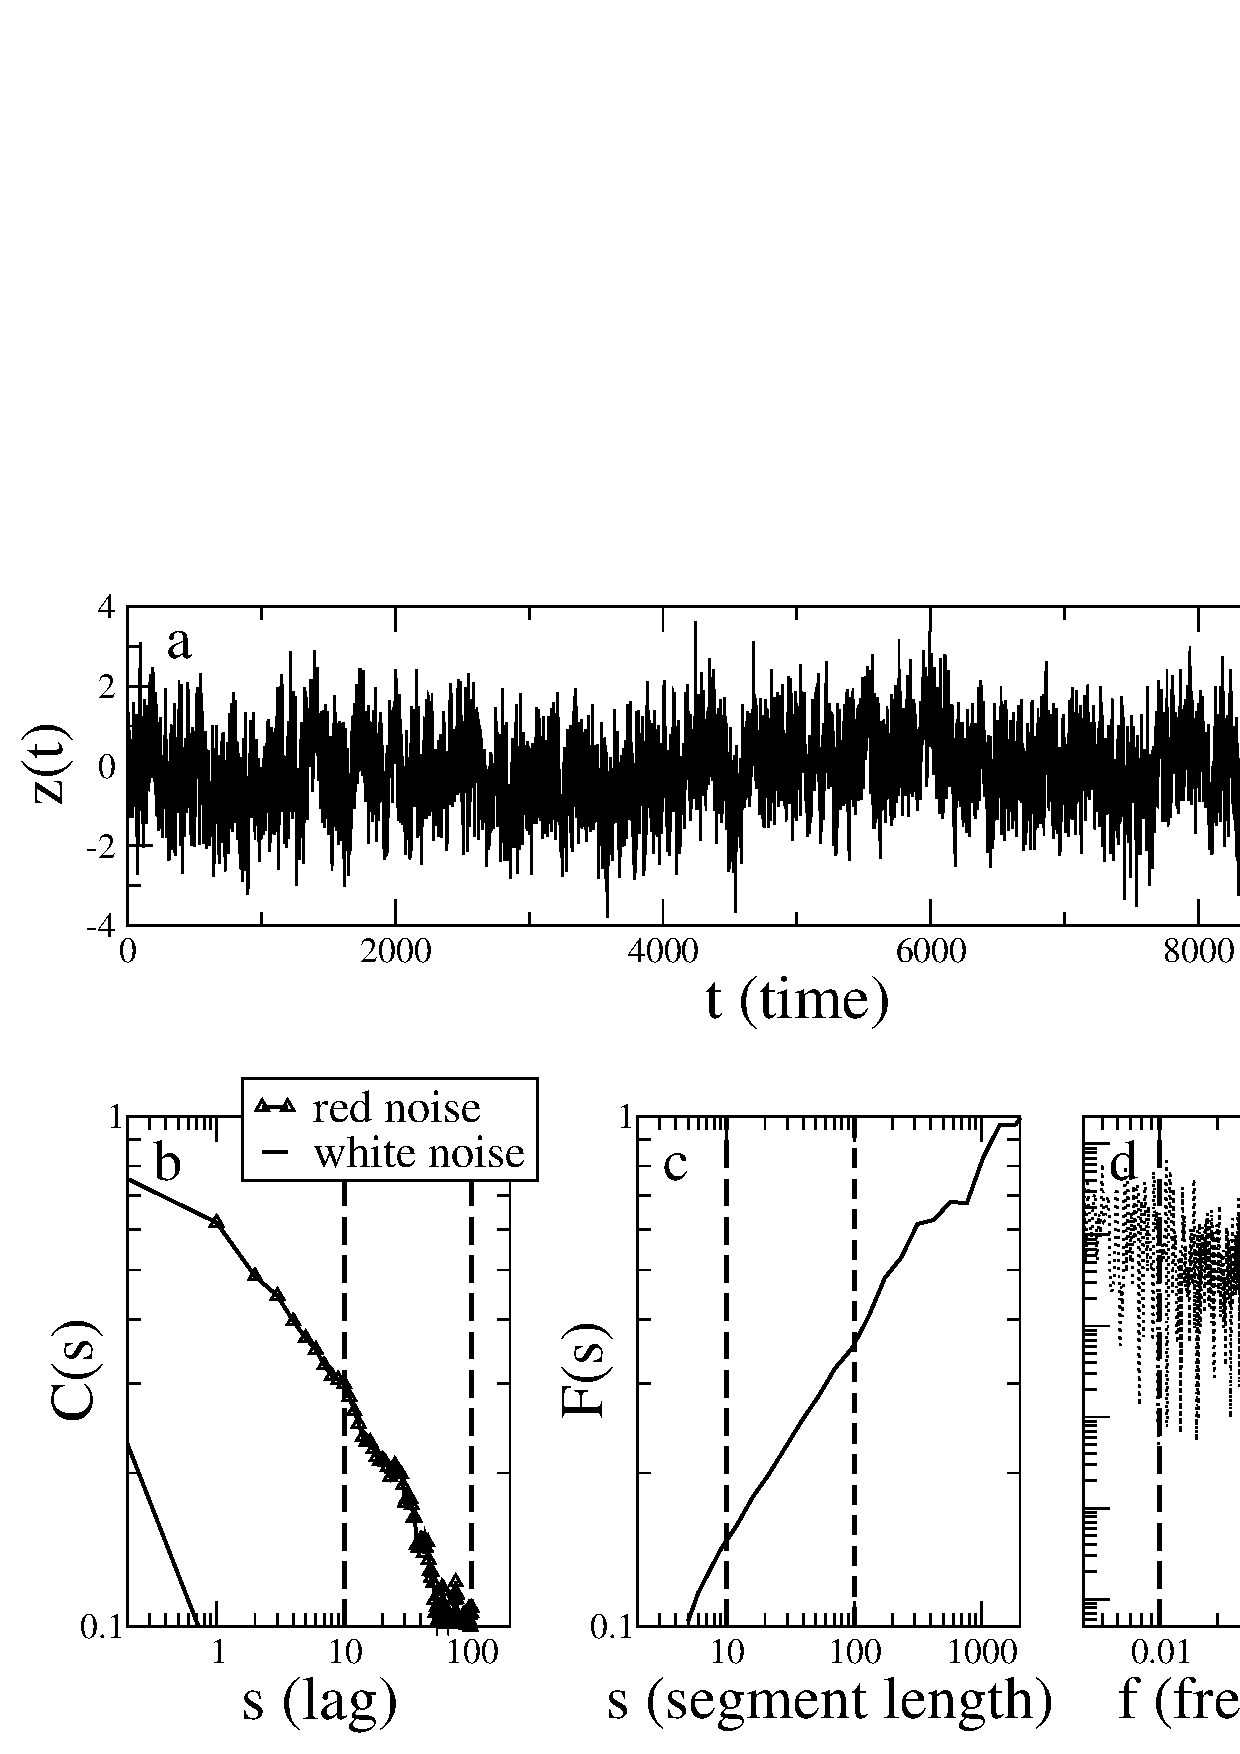
\includegraphics[width = \columnwidth]{fig1_v5}
\caption{Analysis of artificial red noise with scaling exponents 
measured using three different methods. (a) Red noise with a power 
spectrum scaling exponent of 0.85. (b) The ACF of the red noise 
data is calculated for different lags and the exponent (negative slope) 
measured in the range $10\leq s \leq 100$ (dashed lines). 
We note that the ACF(1) indicator ($C(1)$) is 0.64. 
The ACF of a white noise series is also plotted for comparrison, 
in this case $C(s)=0$ for $s\geq 1$ and the exponent is also zero. 
(c) DFA calculated for the data and the exponent (slope) measured 
in the range $10\leq s \leq 100$. (d) The power spectrum of the data, 
and the exponent (negative slope) measured in the frequency range 
$10^{-2} \leq f \leq 10^{-1}$. 
\label{fig1}}
\end{figure}

The DFA scaling exponent ($\alpha$) is measured 
following~\cite{kantelhardt2001}, fig.~\ref{fig1}c. 
Where $F(s)$ is the DFA function of time series $X$, 
with segment length (scale) $s$, we have 
\begin{equation} 
F(s) \sim s^\alpha. \label{DFA_scaling_equation} 
\end{equation} 
In this paper we consistently use an order-2 polynomial 
during the detrending step of DFA. Following the approach 
of~\cite{livina2007}, we measure the DFA exponent in the temporal 
range $10\leq s \leq 100$, which is sensitive to changes in the 
system dynamics similarly to ACF(1).

The power spectrum scaling exponent ($\beta$) is calculated by 
estimating the slope of the power spectrum $S(f)$ of the data, 
plotted on logarithmic axes \cite{bak1988}, from which one can 
obtain $\beta$ via the scaling relationship 
\begin{equation} 
S(f) \sim f^{-\beta}.
\end{equation} 
Here, the power spectrum is approximated by the periodogram, 
obtained from the absolute value of the fast Fourier transform. 
We measure the exponent (slope) inside the frequency range 
$10^{-2} \leq f \leq 10^{-1}$ corresponding to the time range of 
$10$ to $100$ units, to put the technique in agreement with with 
the ACF and DFA methods, as above.

Analytically, the three scaling exponents have the linear relationship:
\begin{equation} 
\alpha = \frac{1+\beta}{2} = 1 - \frac{\gamma}{2} 
\label{exponent_relationships} 
\end{equation} 
in the asymptotic range~\cite{kantelhardt2001}. 
We therefore expect that a measurement of $\beta$ 
could be used in an application where $\alpha$ or $\gamma$ 
are conventionally used, to provide an alternative metric for EWS, 
which may be informative in cases where other indicators fail to 
detect an approaching tipping point. 

\section{PS-indicator applied to artificial data}\label{subsec_artificialdata} 

In order to estimate an early warning signal for a tipping point, 
we calculate
the value of an indicator in a sliding-window of length $N$ 
points along the time axis, in the range $t_1\leq t \leq t_N$, 
then in the range $t_2\leq t\leq t_{N+1}$, and so on, thus 
following the example of~\cite{held2004} where the ACF(1)-indicator 
(a measurement of lag-1 ACF, distinct from the ACF scaling exponent 
$\gamma$) is used. In that paper, the length of the window is chosen 
to be $10\%$ of the length of the time series. In order to quantify 
uncertainties we will consider a range of window lengths. 
We first, however, take a fixed window length of 100 points 
in order to compare our PS-indicator to the ACF(1)-indicator 
used by~\cite{held2004} and the DFA-indicator used by~\cite{livina2007}, 
when applied to artificial data, illustrated in fig.~\ref{fig2}. 
This experiment is in agreement with an equivalent result 
in~\cite{livina2012}.

We construct artificial data of length $10^4$ points by stitching 
together 50 time series of 200 points. To generate each sub-series we use the same method as used for figure~\ref{fig1} 
(see equation \ref{eqn_inverse_fourier}) with values of $\beta$ 
such that the value varies linearly from 0 (no transformation, 
equivalent to white noise) to 2 \cite{makse1996}. We expect, 
therefore, that the PS-indicator $\beta$ will increase linearly 
from 0 to 2. Because of the relationship between the indicators 
we also expect that the DFA-indicator will increase linearly, 
as demonstrated in fig. \ref{fig2}. We have chosen 
this artificial time series, rather than, for example, the 
Ornstein-Uhlenbeck 
process~\cite{hasselmann1976stochastic, ditlevsen2010, ritchie2016},
to provide an example specifically suited to the PS-indicator and  
to reflect the result in \cite{livina2012} 
where this series was used.

\begin{figure}
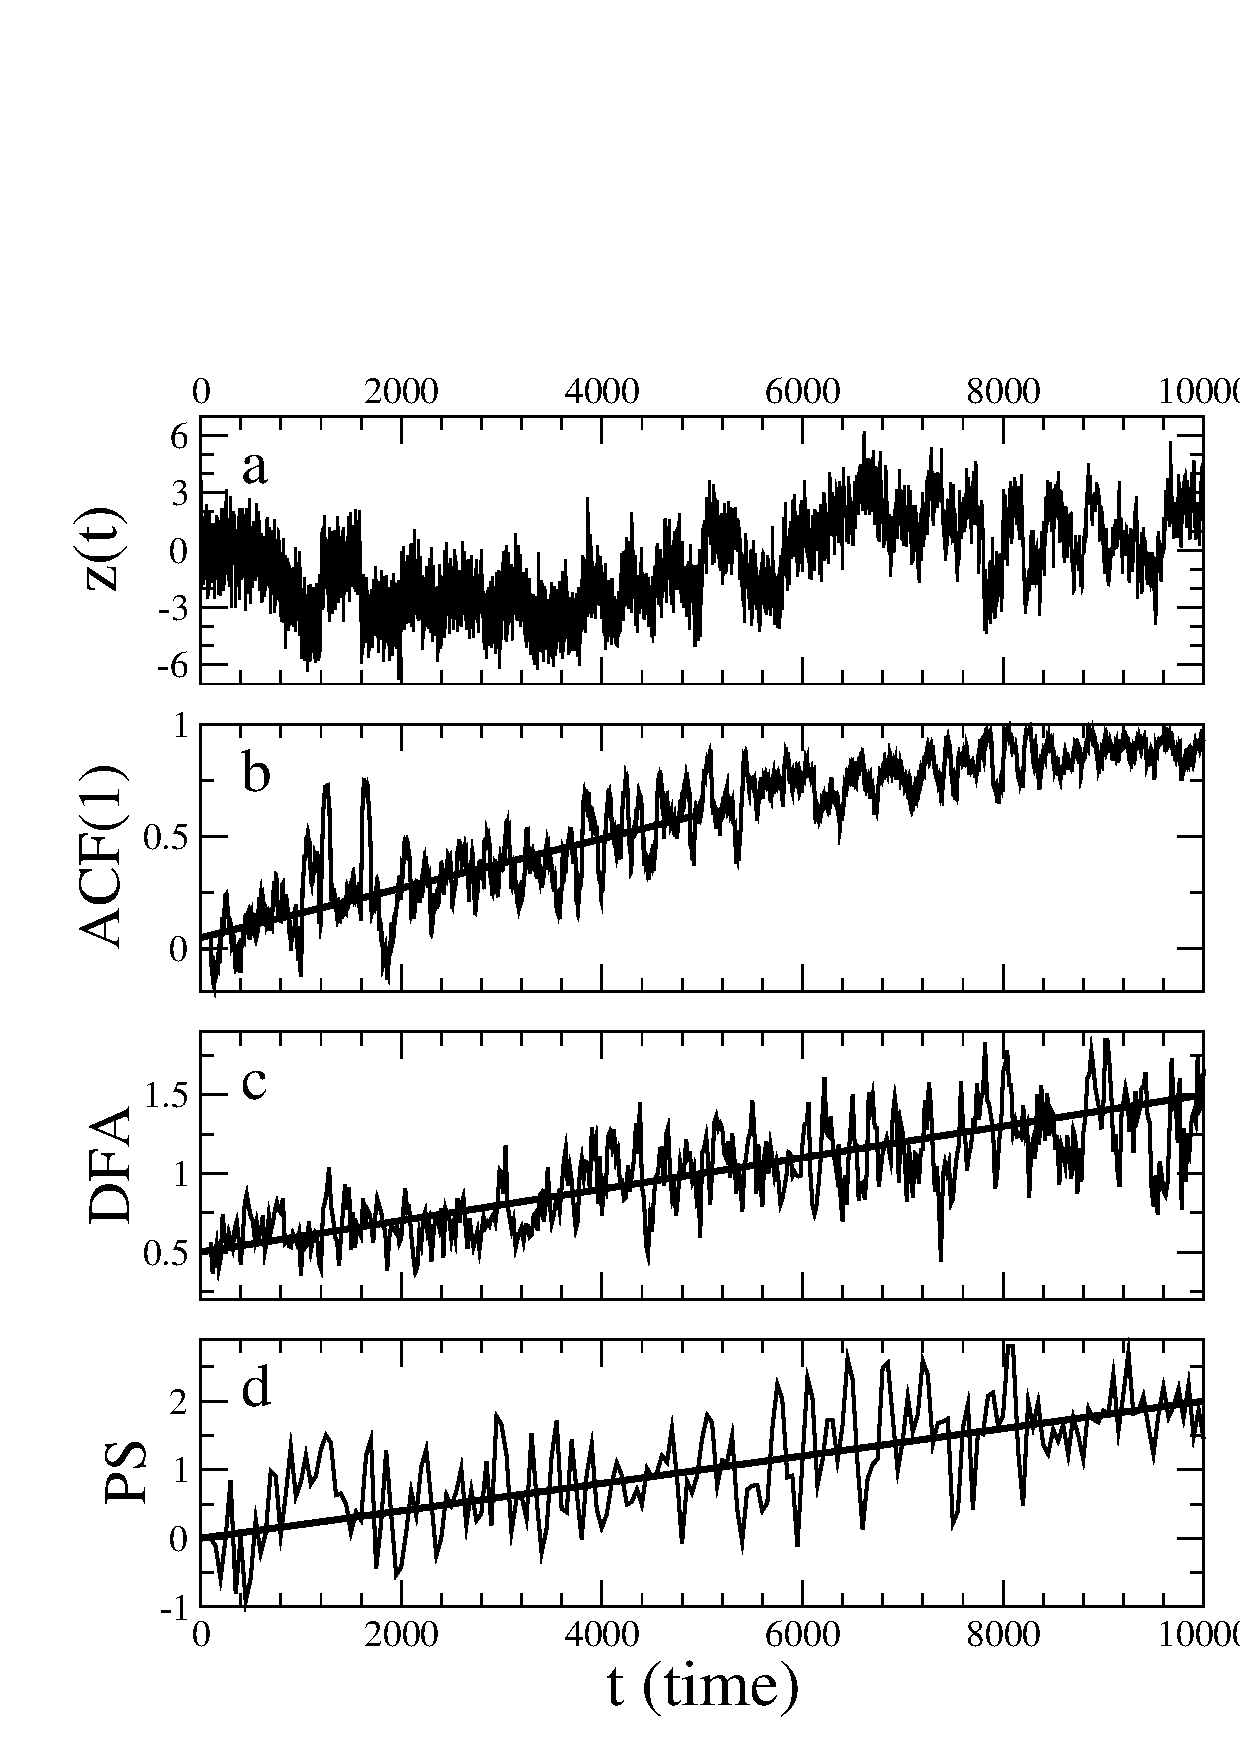
\includegraphics[width = \columnwidth]{fig2_v5}
\caption{Artificial data with ACF(1)-, DFA- and PS-indicators. 
(a) A time series is constructed by concatenating 50 sub-series 
of length 200 where the scaling exponent $\beta$ within each 
sub-series is constant and increases over the whole series from~0 
(white noise) to 2. (b,c,d) The ACF(1)-, DFA- and PS-indicator 
methods are applied with window size 100. As the PS-indicator 
increases from 0 to 2, the ACF(1)-indicator increases from 0 to 1, 
and the DFA scaling exponent $\alpha$ increases from 0.5 to 1.5. 
Lines are added to show the linear trends; note that the 
ACF(1)-indicator does not increase linearly as it approachs~1. 
\label{fig2}}
\end{figure}

\section{PS-indicator applied to model data} \label{sec_modeldata}

We now apply the PS-indicator to a system including a bifurcation point, 
expecting that we will observe behaviour comparable to the ACF(1)- 
and DFA-indicators. We use a typical bifurcating system described 
by the stochastic differential equation 
\begin{equation} 
\dot{z}(t) = -\frac{\partial}{\partial z}\left(z^4 + 
\left(3-\frac{t}{200}\right)z^2\right) + \sigma\eta_t, 
\label{pitchfork_eqn} 
\end{equation} 
where $\sigma=0.05$ and the $\eta_t$ are independent samples from a 
Gaussian distribution. Equation \ref{pitchfork_eqn} is integrated 
numerically with a time step of $\delta t$ = 0.05 from $t=1$ to $t=1000$, 
and sampled with $\Delta t = 1$. In the range $t<600$ the system has 
a single stable node $z=0$, the system then bifurcates after $t=600$ 
into a double-well potential with stable nodes at $z=\pm 0.05\sqrt{t-600}$, 
$z=0$ becomes unstable.

The system is integrated 100 times to produce 100 time series of 
length 1000, see fig. \ref{fig3}a. The EWS indicators are then applied 
to the 100 time series and the mean of all 100 indicator series 
is plotted with error bars of one standard deviation. We have 
performed this with the ACF(1)- and DFA-indicators 
(fig.~\ref{fig3}b,c) and the new PS-indicator (fig.~\ref{fig3}d). 
The ACF(1)-indicator provides a clear EWS as expected, there is 
a definite increasing trend starting at around $t=400$. 
We see a similar trend with the PS-indicator, 
so the validity of the PS-indicator as an EWS is illustrated 
in principle. However, this indicator has high variance, 
and the mean at 
$t=600$ does not rise above the upper error bound 
(one standard deviation, $1\sigma$) 
for $t<500$. This means that at the early development of the 
trend in the PS-indicator in live monitoring of
this dynamical system, the rise of the indicator may be attributed
to its stochastic variability.

It is necessary to note that the pitchfork 
bifurcation was chosen because in this case
ACF(1) provides a clear EWS. Therefore, 
it is a good testbed for the PS-indicator, by analogy.  

\begin{figure}
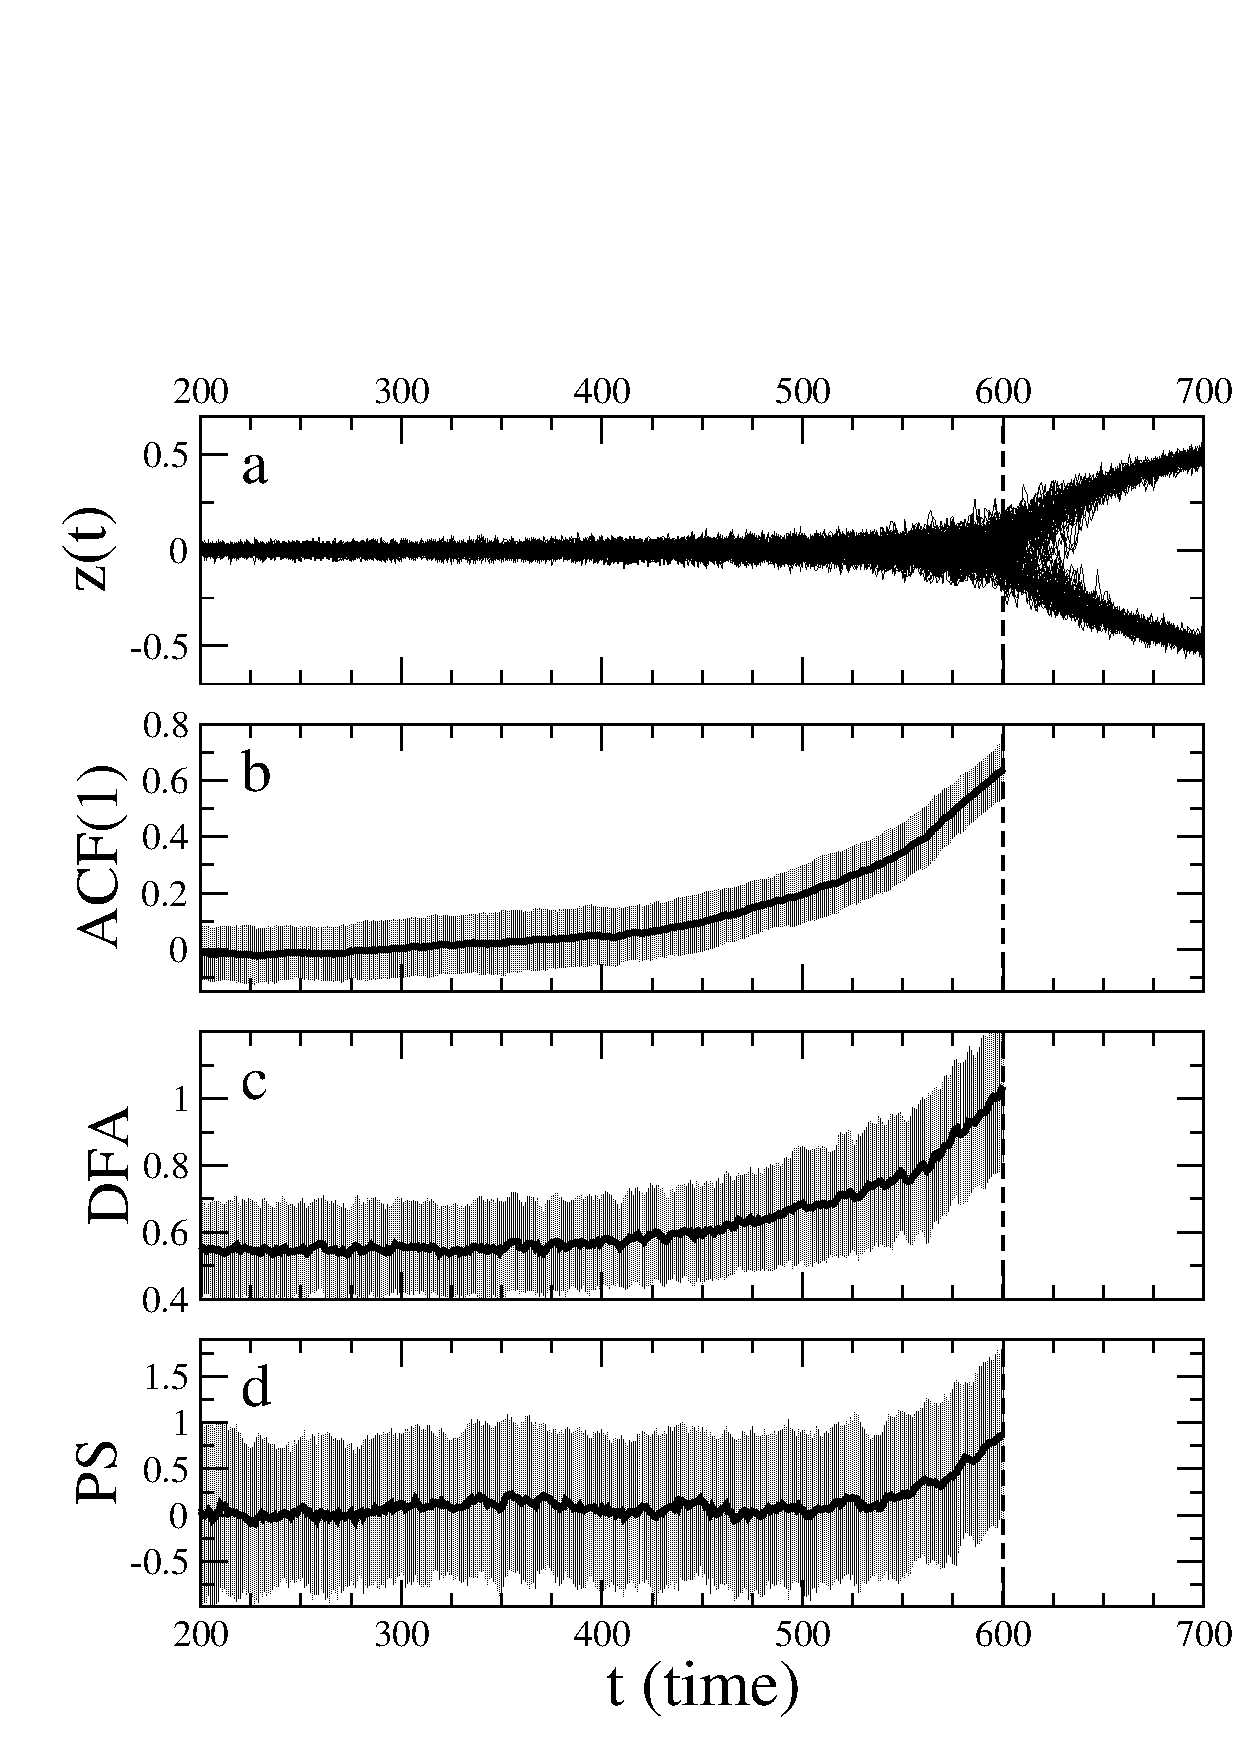
\includegraphics[width = \columnwidth]{fig3_v4}
\caption{ACF(1)-, DFA- and PS-indicators applied to model data. 
(a) Data from 100 runs of the model (see eq. \ref{pitchfork_eqn}); 
(b,c,d) The mean ACF(1), DFA and PS-indicators (window size 100), 
with error bars of one standard deviation. The values of all the 
indicators begin to rise before the bifurcation, as expected, 
at around $t=500$, although it is most noticeable for the 
ACF(1)-indicator. \label{fig3}}
\end{figure}

\section{PS-indicator applied to tropical cyclones}\label{sec_cyclonedata}

We now apply the PS-indicator to data from a real geophysical system. 
We use hourly, one-dimensional sea-level pressure data from observation 
stations within 2km of the landfall locations of 14 tropical cyclones. 
The data is obtained from the HadISD2005 dataset, available from the 
UK~MetOffice \cite{HadISD_smith,HadISD_dunn} (see \cite{HadISDwebsite}) selected for 
falling close to one of these stations, and being ranked category 
4 or 5, using the Saffir-Simpson scale, at the time of landfall. 
The 14 selected are: Atlantic hurricanes Andrew (1992), Opal (1995), 
Floyd (1999), Charley (2004), Frances (2004), Jeanne (2004), Katrina (2005), 
Rita (2005), Ivan (2006) and Ernesto (2006); typhoons Zeb (1998), 
Megi (2010) and Flo (1990); and Cyclone Hudhud (2014).

We do not attempt to provide an analytical description of the tropical 
cyclone data and it does not appear to contain a bifurcation in the 
same sense as the pitchfork bifurcation (eq.~\ref{pitchfork_eqn}, 
fig.~\ref{fig3}). However, there is a transitional tipping point 
in the sense that the pressure drops suddenly when the cyclone passes 
over, and this most likely affects the dynamics of the fluctuations, 
providing a detectable EWS. We center the time series for each cyclone 
on the minimum pressure value (fig. \ref{fig4}a), which time we call 
$t=0$. This cannot be called analogous to the bifurcation point at 
$t=600$ in the pitchfork bifurcation example, but is a common feature 
which is convenient to use for the purpose of comparison.

We use the same method as used for the bifurcating model data in the 
previous section, applying the indicator in a sliding window of 100 
points to all 14 time series and plotting the mean of all 14 indicator 
series, with error bars of one standard deviation. Again, we apply both 
the ACF(1)- and DFA-indicators (fig. \ref{fig4}b,c) and the new 
PS-indicator (fig. \ref{fig4}d). The ACF(1)-indicator, 
in this case, does not appear to provide a clear EWS, 
whereas the PS-indicator does show an increasing trend starting at 
around 50 hours before the minimum pressure.

\begin{figure}
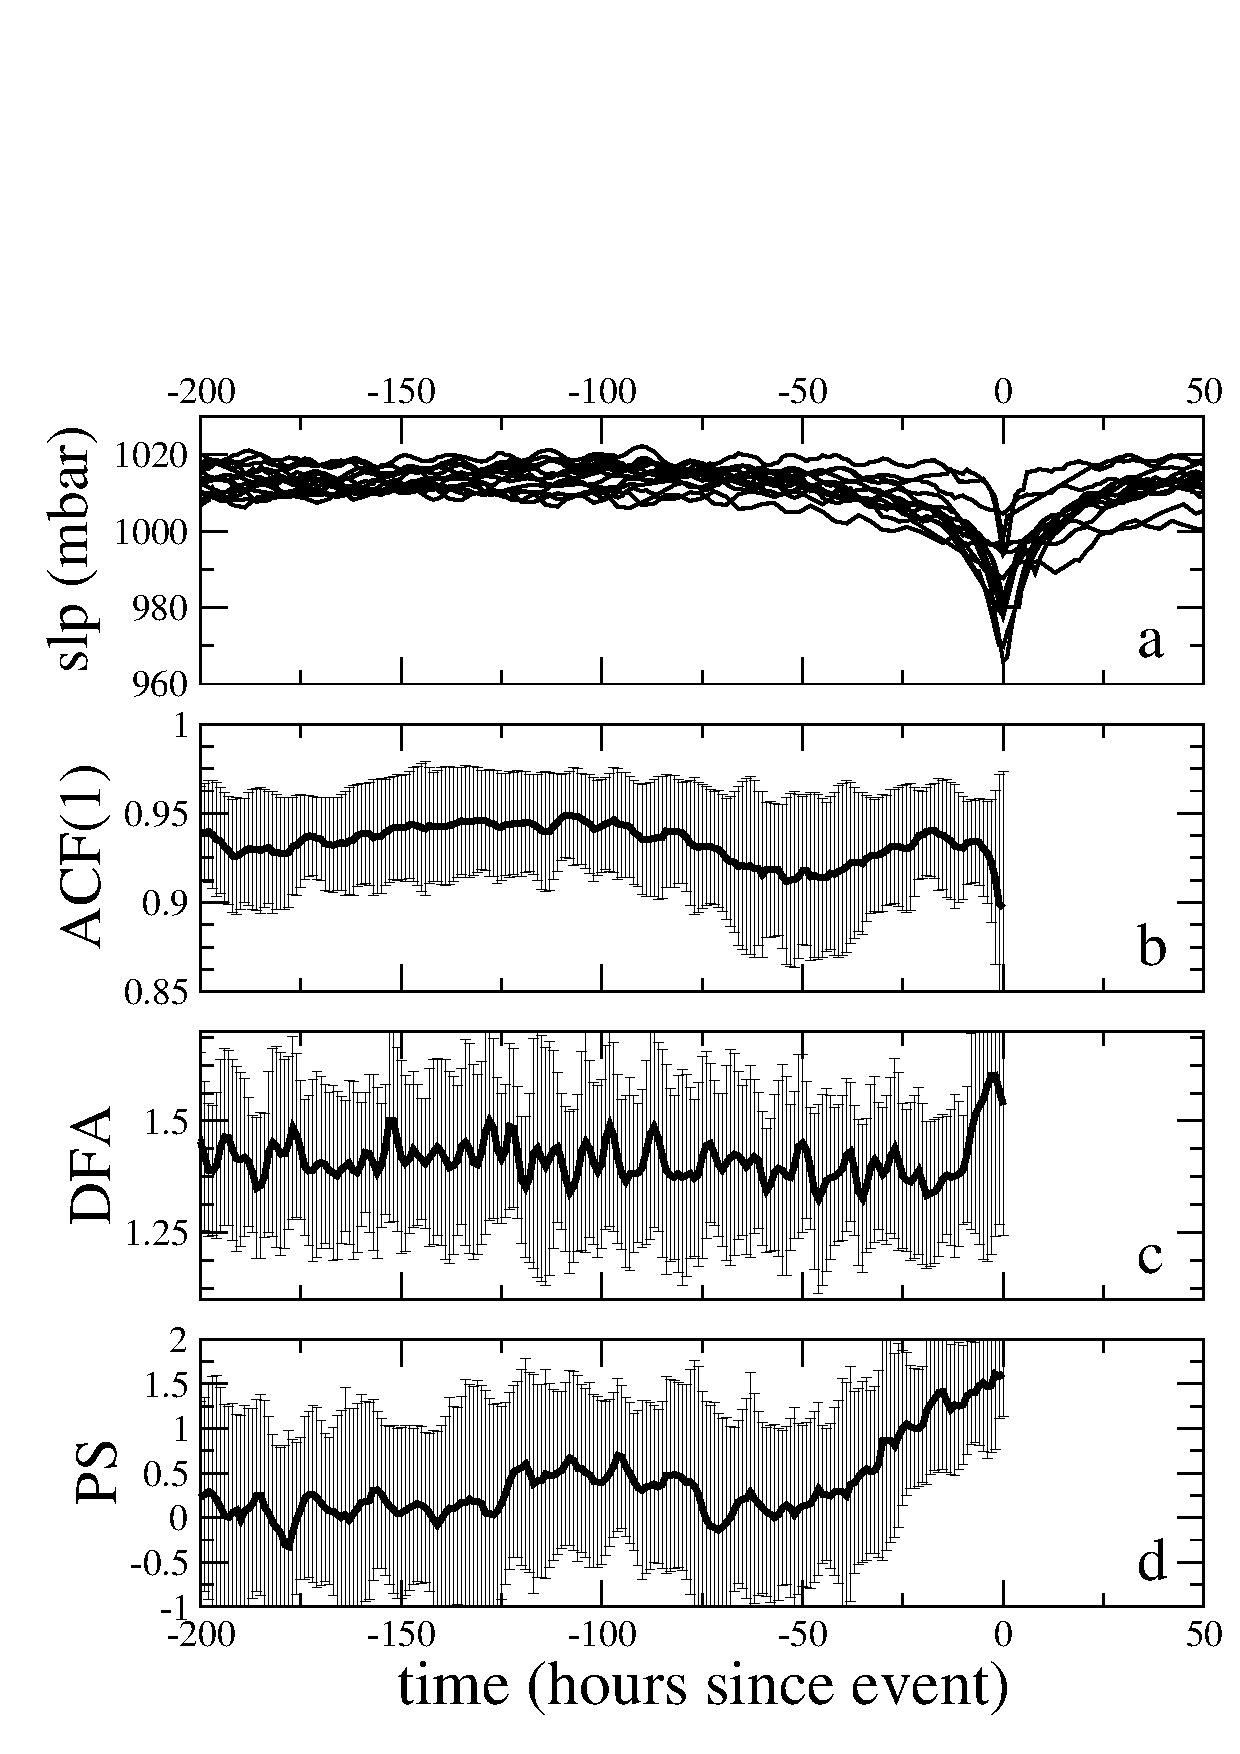
\includegraphics[width = \columnwidth]{fig4_v4}
\caption{ACF(1)-, DFA- and PS-indicator methods applied to sea-level 
pressure data. (a) Data from the 14 tropical cyclones. 
(b,c,d)~The mean ACF(1)-, DFA- and PS-indicators (window size 100), 
with error bars of 1 standard deviation. The ACF(1)-indicator does 
not provide a clear EWS in this case. The DFA-indicator shows a 
noticable increasing trend just before the event. The PS-indicator 
appears to rise around 50 hours before the cyclone event. \label{fig4}}
\end{figure}

\section{Sensitivity of the method to window size} \label{sec_sensitivity}

The method described provides an estimate of the changes in the PS 
scaling exponent in a window of 100 points. It is desirable to use 
a very large number of points to give an accurate estimate of the 
scaling exponent from the periodogram, less sensitive to periodic 
oscillations in the data and also with less variability over time. 
However, one must compromise this since the window size must 
correspond to the time scale of the phenomenon under investigation; 
of course there is also a limit imposed by the length of the 
time series data. We require a window size such that the indicator 
variance is significantly small that we can see the EWS, but that 
the rise in the indicator value before the tipping event is large 
enough so that we can recognise it as an EWS.

It is useful to produce a contour plot of the mean value of the 
indicator over time, with window-size on the $y$-axis. 
We expect that the EWS apparently becomes stronger with decreasing 
window size, above a certain size where the variability becomes 
so large that it is not possible to detect an EWS. In this way, 
we make a subjective choice as to the optimum window size to use 
in each context and assume that we can reasonably expect that this 
choice can be applied to new data from the same source.

In fig. \ref{fig5} we see that there is an increasing trend in the 
PS-indicator towards the end of the time series with almost 
all window sizes. The exceptions occur periodically where the window 
size is approximately $12n\pm 1$ for integer $n$, using these window 
sizes the indicator is approximately 1.5 over the whole series. 
Note that the most obvious signals occur with window sizes 102, 
114 and 126. Using larger values (e.g. 174) the useful variability 
in the indicator is smoothed out so that the trend towards the end 
of the series is less obvious.

The periodic pattern in the contour plot (fig.~\ref{fig5}) is 
caused by an oscillation with period $\approx$ 12 hours in 
the sea-level pressure data, likely caused by tidal influences. 
In this context it is therefore essential to consider 
the sensitivity of the method to the window size parameter, 
as we have done here.

\begin{figure}
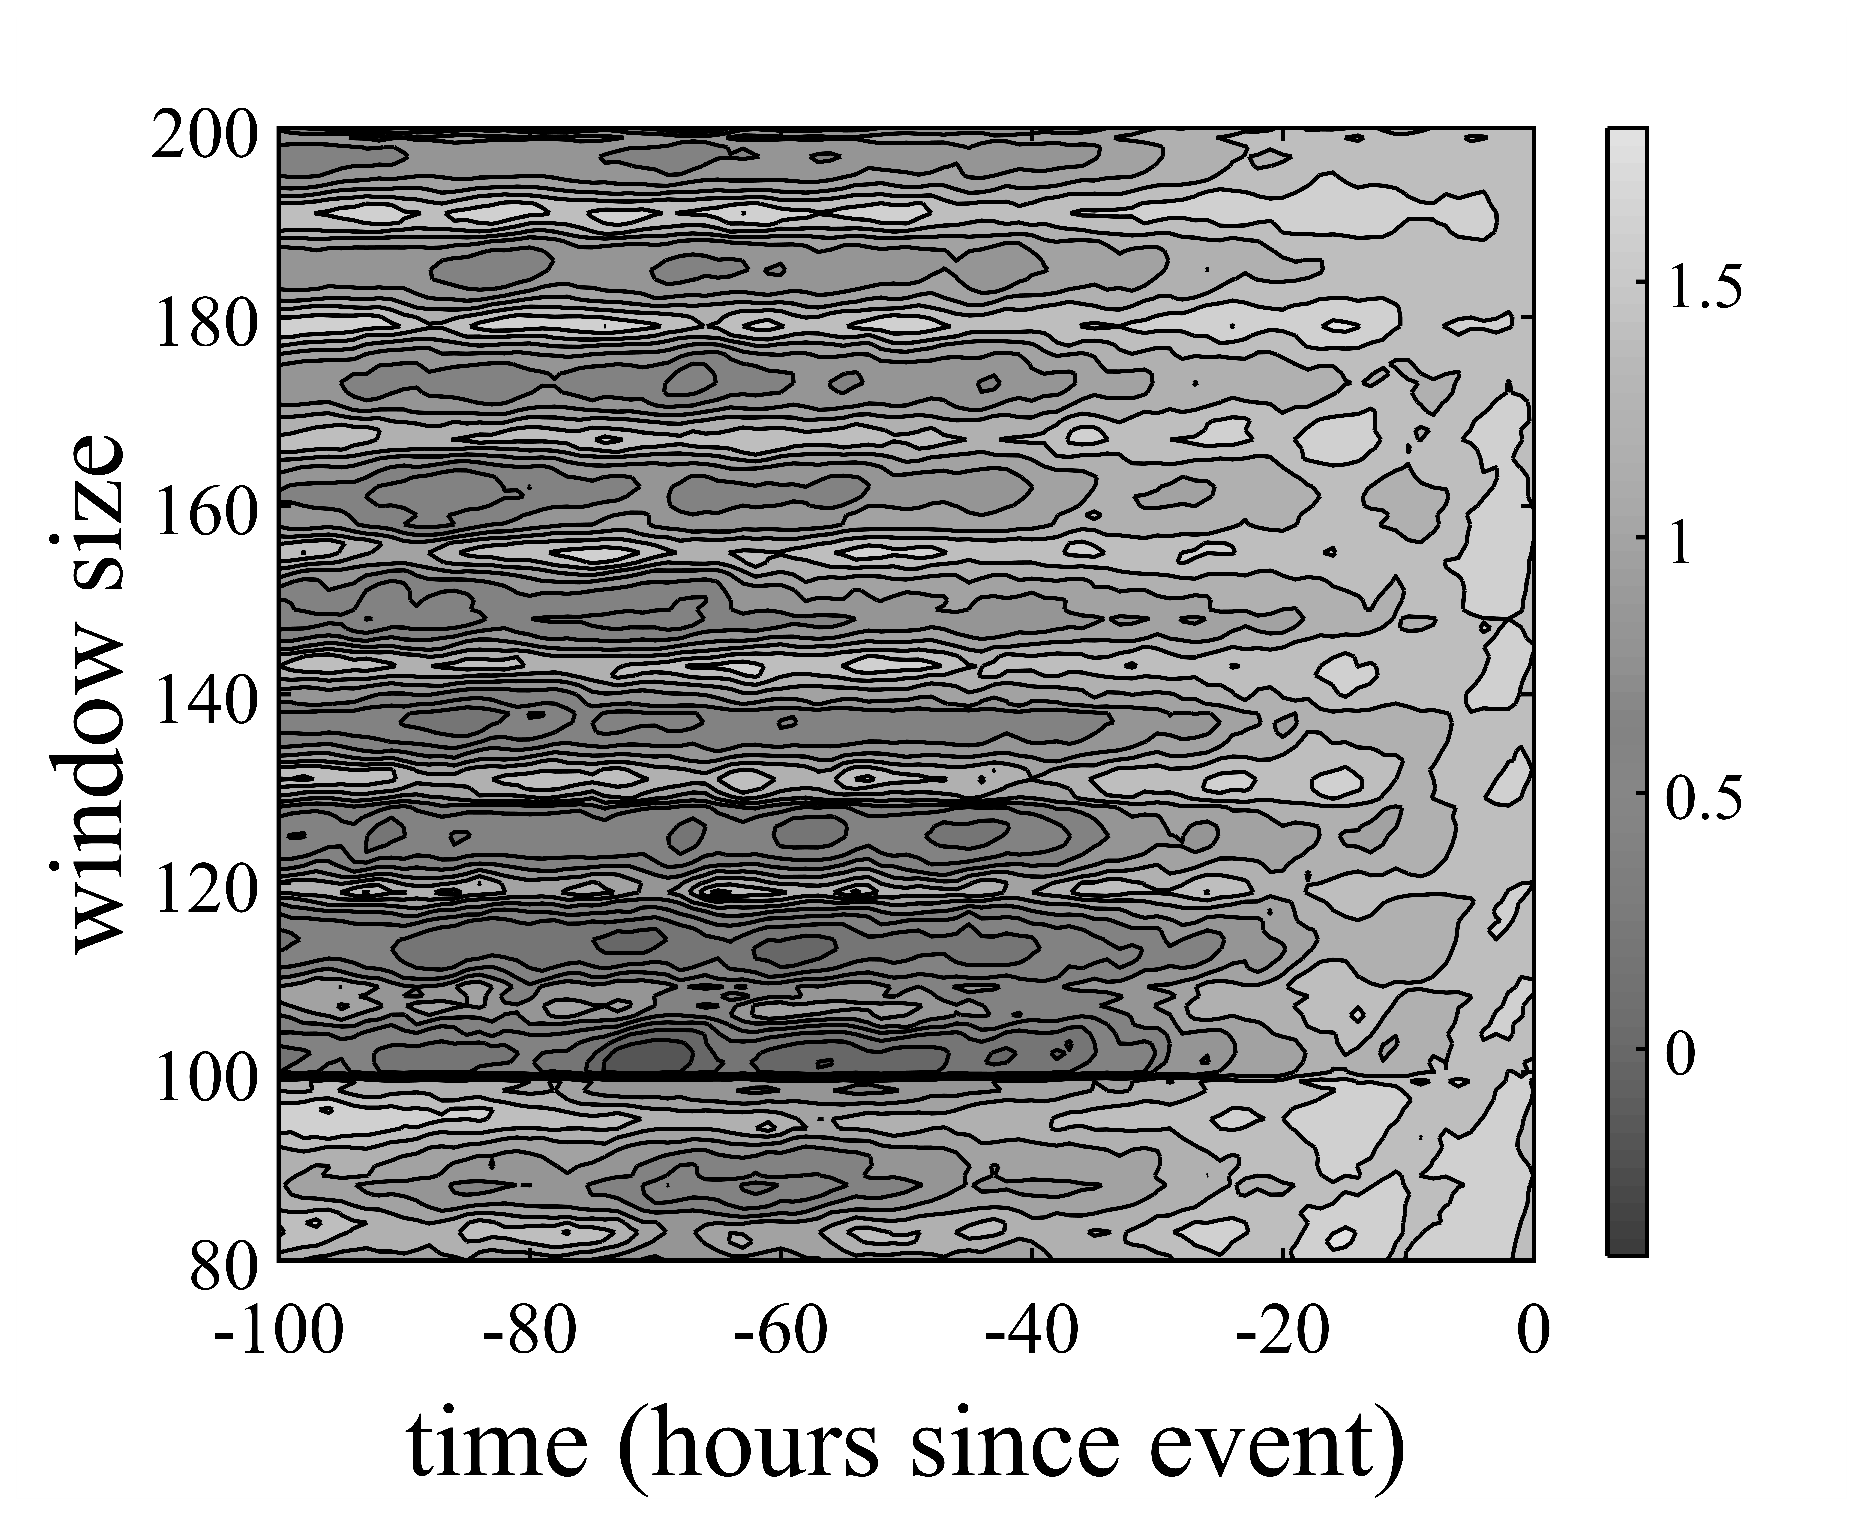
\includegraphics[width = \columnwidth]{fig5_v6}
\caption{Mean PS-indicator for tropical cyclone data 
(see fig.~\ref{fig4}) calculated using window sizes from 
80 to 200. The PS-indicator appears to rise around 40 
hours before the cyclone event in almost all cases, 
the exceptions occur when the window size has the value $12n\pm 1$, 
in these cases the indicator is high (approximately $1.5$) 
over the entire series. \label{fig5}}
\end{figure}

\section{Discussion}\label{sec_discussion}
We have developed a novel indicator of EWS for tipping points 
in dynamical systems by estimating the power-law decay rate of 
the power spectrum in a sliding window. We have applied this 
PS-indicator to three time series: an artificial example of 
increasing scaling exponent; a model including a bifurcation; 
and sea-level pressure data measured at the landfall sites of 
14 tropical cyclones.

In the case of high-frequency sampling
of data, it is likely that the autocorrelation would be fluctuating 
at very high level (close to maximal value~1) and not providing any 
meaningful EWS information. In such cases, for applying any EWS indicator
based on scaling properties (ACF, DFA or PS), it would be useful to 
pre-process the data with 
some aggregation or averaging, similarly to~\cite{held2004}. 
However, this issue is not specific to the 
new PS-indicator. Moreover, in many cases a time series is pre-processed 
before calculating EWS indicators (for instance, using Gaussian filter
or moving average), which immediately changes the absolute value of
autocorrelation and other scaling exponents. This means that the critical 
value of autocorrelation changes, and it is no longer bounded 
by the critical
value~1. In such cases, the increasing trend of an EWS indicator is more
informative than its values, which is a shortcoming of the approach with 
such data pre-processing. So far, its impact on the EWS 
indicators has not been studied, either in the context of analytical 
rigour or in the context of proximity to a tipping point; 
this must be a topic of further research in the area of 
early warning signals.

On the other hand, the length of the series (always
finite and often imposing finite-size-effect challenges) may be problematic
in case of estimation, for instance, variance in fixed-size windows. 
As was demonstrated in Fig.2 (middle panel) 
of~\cite{livina2012}, using
fixed-size window in studying a dataset with increasing scaling exponent 
may generate a decreasing variance indicator. 


We have found that the PS-indicator behaves similarly to the 
previously used ACF(1)- and DFA-indicators applied to the model 
data, but with larger variance, which limits its usefulness in 
situations where the model cannot be observed multiple times. 
When applied to the sea-level pressure data, the ACF(1)- and 
DFA-indicators do not appear to provide an EWS. However, the 
PS-indicator clearly does begin to increase around 50 hours 
before the lowest pressure, about the same point that the 
decreasing trend in pressure becomes visible, suggesting that 
it can provide a detectable EWS in this context. 

The approaching cyclone is chosen as an example 
of a system which 
has not previously been studied using tipping-point 
EWS methods, and for which the dynamics of the system are unknown, 
thus providing a ``blind'' experiment. The passing cyclone is not 
modelled as a phase transition, and it is not known whether 
there exists a critical point such that we might claim universality 
of the scaling exponents. Rather, we have a time series which 
superficially resembles other geophysical tipping-point examples 
(see~\cite{dakos2008}), thus we wish to 
experiment with our existing EWS methods, and then compare the 
performance of our new indicator. 
In this sense, it is an heuristic 
investigation of the properties of the new technique, with 
comparison with similar methods. We report our findings to facilitate
further investigation of this technique.


We conclude that the PS-indicator is a novel and useful technique 
which behaves similarly to the related ACF(1)- and DFA-indicators 
in idealised systems. It also shows signs of providing a useful 
EWS for the real geophysical system of impending tropical cyclones, 
where the ACF(1)-indicator fails. 

\bibliography{bibliography_v2.bib}

\end{document}
